\documentclass[draft,jgrga]{agutexSI2019}

\usepackage{xr}
\externaldocument{manuscript_agu_rev1}

\makeatletter
\def\@makecol{\setbox\@outputbox
     \vbox{\boxmaxdepth \maxdepth
\ifdim\ht\dbltopins<1pt\else\unvbox\dbltopins\fi
     \unvbox\@cclv
\ifdim\ht\dblbotins<1pt\else\unvbox\dblbotins\fi%
\ifvoid\footins\else\vskip\skip\footins\footnoterule\unvbox\footins\fi
%\vss
\vskip 0pt plus 1fil minus \maxdimen
}%
%\global\savefigandtabnumber\figandtabnumber
%\global\advance\savefigandtabnumber by 1 %% Because loop stops one short
                                         %% of the total number of figs
\global\savedblfigandtabnumber\dblfigandtabnumber
   \xdef\@freelist{\@freelist\@midlist}\gdef\@midlist{}\@combinefloats
   \setbox\@outputbox\vbox to\@colht{\boxmaxdepth\maxdepth
   \@texttop\dimen128=\dp\@outputbox\unvbox\@outputbox
   \vskip-\dimen128\@textbottom}%
   \global\maxdepth\@maxdepth}
\makeatother

 \usepackage{graphicx}

%  Uncomment the following command to allow illustrations to print
%   when using Draft:
 \setkeys{Gin}{draft=false}

\authorrunninghead{KUMA ET AL.}

\titlerunninghead{SHIP-BASED LIDAR EVALUATION OF SO LOW CLOUDS}

\authoraddr{Corresponding author: P. Kuma, Institute for Atmospheric and Environmental Sciences, Goethe University Frankfurt, Altenhöferallee 1, Frankfurt am Main, 60438, Hesse, Germany. (peter@peterkuma.net)}

\begin{document}

%\includegraphics{agu_pubart-white_reduced.eps}

\title{Supporting Information for "Ship-based lidar evaluation of Southern Ocean low clouds in the storm-resolving general circulation model ICON, and the ERA5 and MERRA-2 reanalyses"}

\authors{Peter Kuma\affil{1,2,3,4}, Frida A.-M. Bender\affil{1,2}, Adrian J. McDonald\affil{3}, Simon P. Alexander\affil{5,6}, Greg M. McFarquhar\affil{7,8}, John J. Cassano\affil{9,10,11}, Graeme E. Plank\affil{3}, Sean Hartery\affil{3}\thanks{Current affiliation: Department of Physics \& Atmospheric Science, Dalhousie University, Halifax, Canada}, Simon Parsons\affil{3}\thanks{Current affiliation: New South Wales Department of Planning and Environment, Sydney, New South Wales, Australia}, Sally Garrett\affil{12}, Alex J. Schuddeboom\affil{3}, and Anna Possner\affil{4}}

\affiliation{1}{Department of Meteorology (MISU), Stockholm University, Stockholm, Sweden}
\affiliation{2}{Bolin Centre for Climate Research, Stockholm University, Stockholm, Sweden}
\affiliation{3}{School of Physical and Chemical Sciences, University of Canterbury, Christchurch, Aotearoa/New Zealand}
\affiliation{4}{Institute for Atmospheric and Environmental Sciences, Goethe University Frankfurt, Frankfurt am Main, Hesse, Germany}
\affiliation{5}{Australian Antarctic Division, Kingston, Tasmania, Australia}
\affiliation{6}{Australian Antarctic Program Partnership, Institute for Marine and Antarctic Studies, University of Tasmania, Hobart, Tasmania, Australia}
\affiliation{7}{Cooperative Institute of Severe and High Impact Weather Research and Operations, University of Oklahoma, Norman, OK, USA}
\affiliation{8}{School of Meteorology, University of Oklahoma, Norman, OK, USA}
\affiliation{9}{Cooperative Institute for Research in Environmental Sciences, University of Colorado, Boulder, CO, USA}
\affiliation{10}{National Snow and Ice Data Center, University of Colorado, Boulder, CO, USA}
\affiliation{11}{Department of Atmospheric and Oceanic Sciences, University of Colorado, Boulder, CO, USA}
\affiliation{12}{New Zealand Defence Force, Wellington, Aotearoa/New Zealand}

\begin{article}

\noindent\textbf{Contents of this file}
\begin{enumerate}
\item Figure S1
\item Figure S2
\item Figure S3
\item Figure S4
\item Figure S5
\end{enumerate}

\end{article}
\clearpage

\begin{figure}[p!]
\centerline{
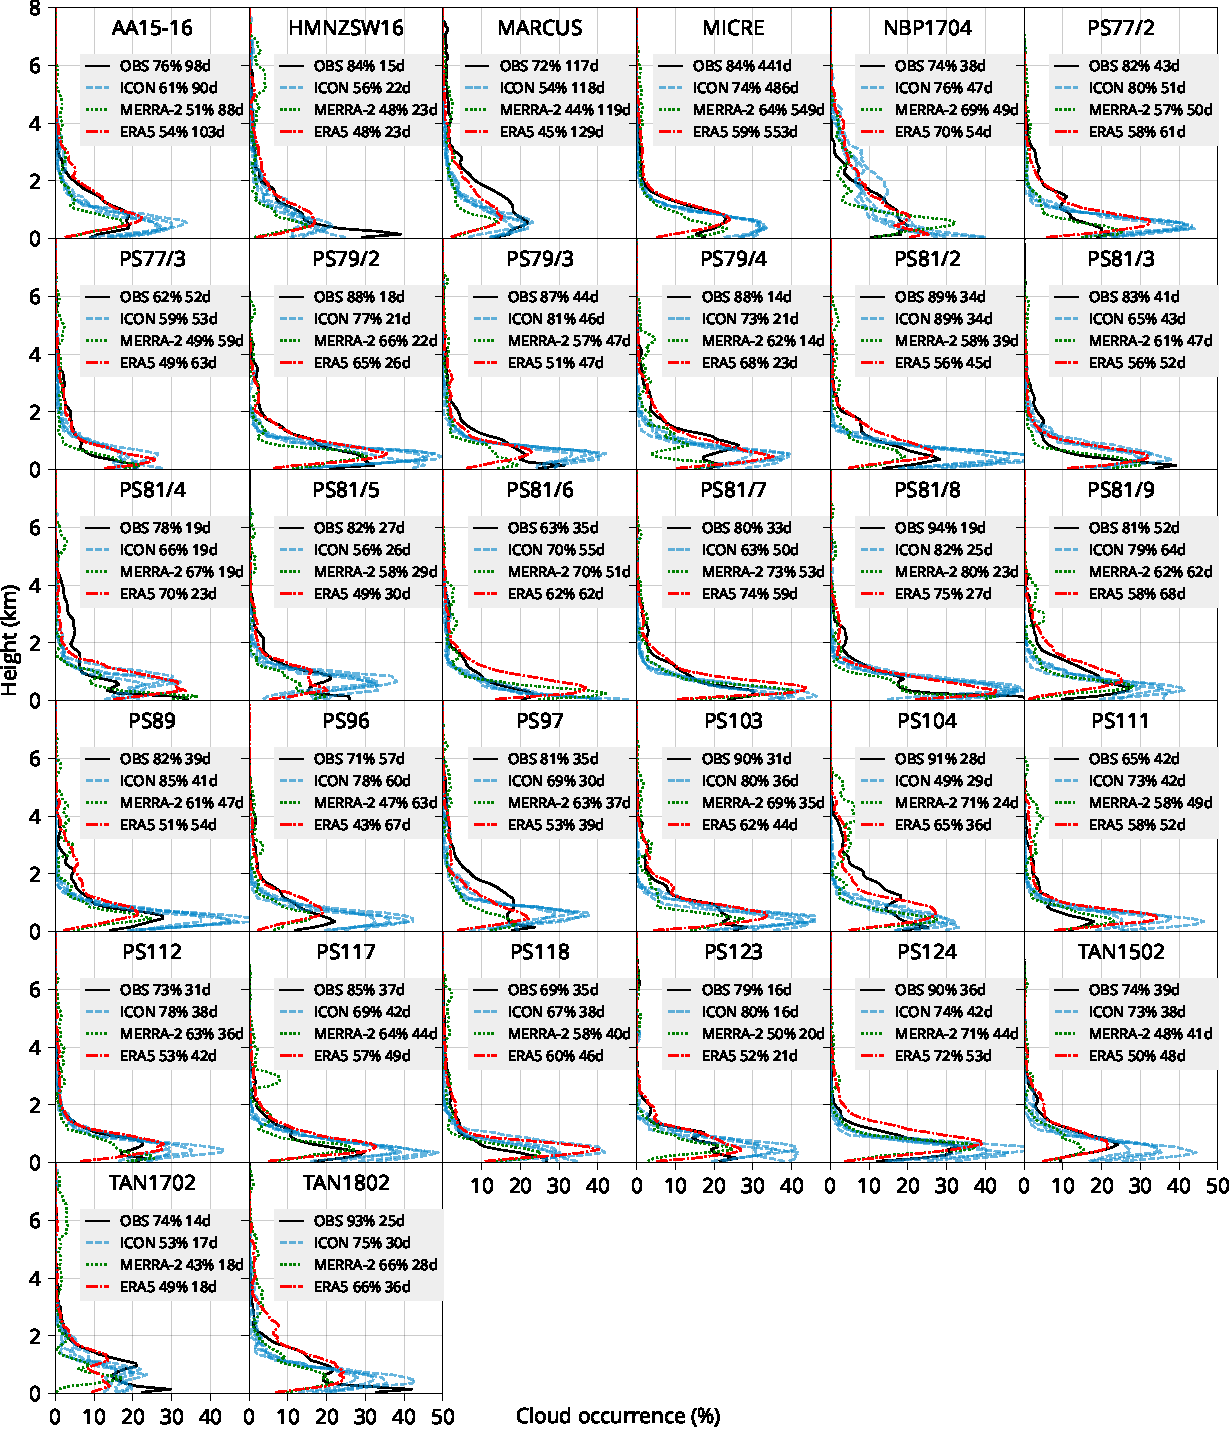
\includegraphics[width=0.95\textwidth]{img/cl.pdf}
}
\caption{
Cloud occurrence by height for the 31 voyages and one sub-Antarctic station (MICRE) in observations (O) and simulated by the ALCF from the ICON model (I), MERRA‐2 (M), and ERA5 reanalysis data (E). The numbers in the legend indicate the total cloud fraction and the number of days of data. Multiple lines of ICON profiles are for each of the four years of model data available.
}
\label{fig:cloud-occurrence-panel}
\end{figure}

\begin{figure}[p!]
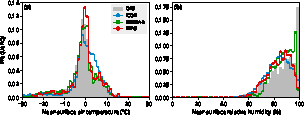
\includegraphics[width=\textwidth]{img/stats_hist_surf.pdf}
\caption{
Histograms of near-surface \textbf{(a)} air temperature and \textbf{(b)} relative humidity at radiosonde launch locations in the observations and the corresponding locations and times in the models. Only locations south of 40°S are included.
}
\label{fig:stats-hist-surf}
\end{figure}

\begin{figure}[p!]
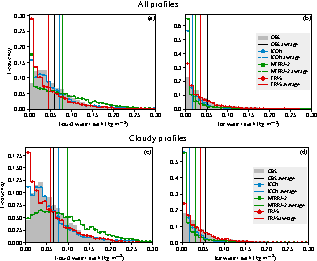
\includegraphics[width=\textwidth]{img/stats_hist_si.pdf}
\caption{
Histograms and averages of \textbf{(a, c)} liquid water path, and \textbf{(b, d)} ice water path in CERES SYN1deg observations (OBS), ICON,
MERRA-2, and ERA5 for \textbf{(a, b)} all and \textbf{(c, d)} cloudy profiles. All campaigns are weighted equally. The statistics are calculated from daily mean values corresponding to each time step and geographical location of the voyage tracks and stations.
}
\label{fig:stats-hist-si}
\end{figure}

\begin{figure}[t]
\centerline{
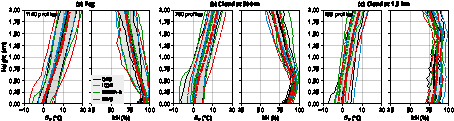
\includegraphics[width=1.2\textwidth]{img/rs_thetav_hur_cloud.pdf}
}
\caption{
The same as Fig.~\ref{fig:potential-temperature}, but only for profiles that contain \textbf{(a)} fog, \textbf{(b)} cloud at 500~m, and \textbf{(c)} cloud at 1.5~km.
}
\label{fig:rs-thetav-hur-cloud}
\end{figure}

\begin{figure}[t]
\centerline{
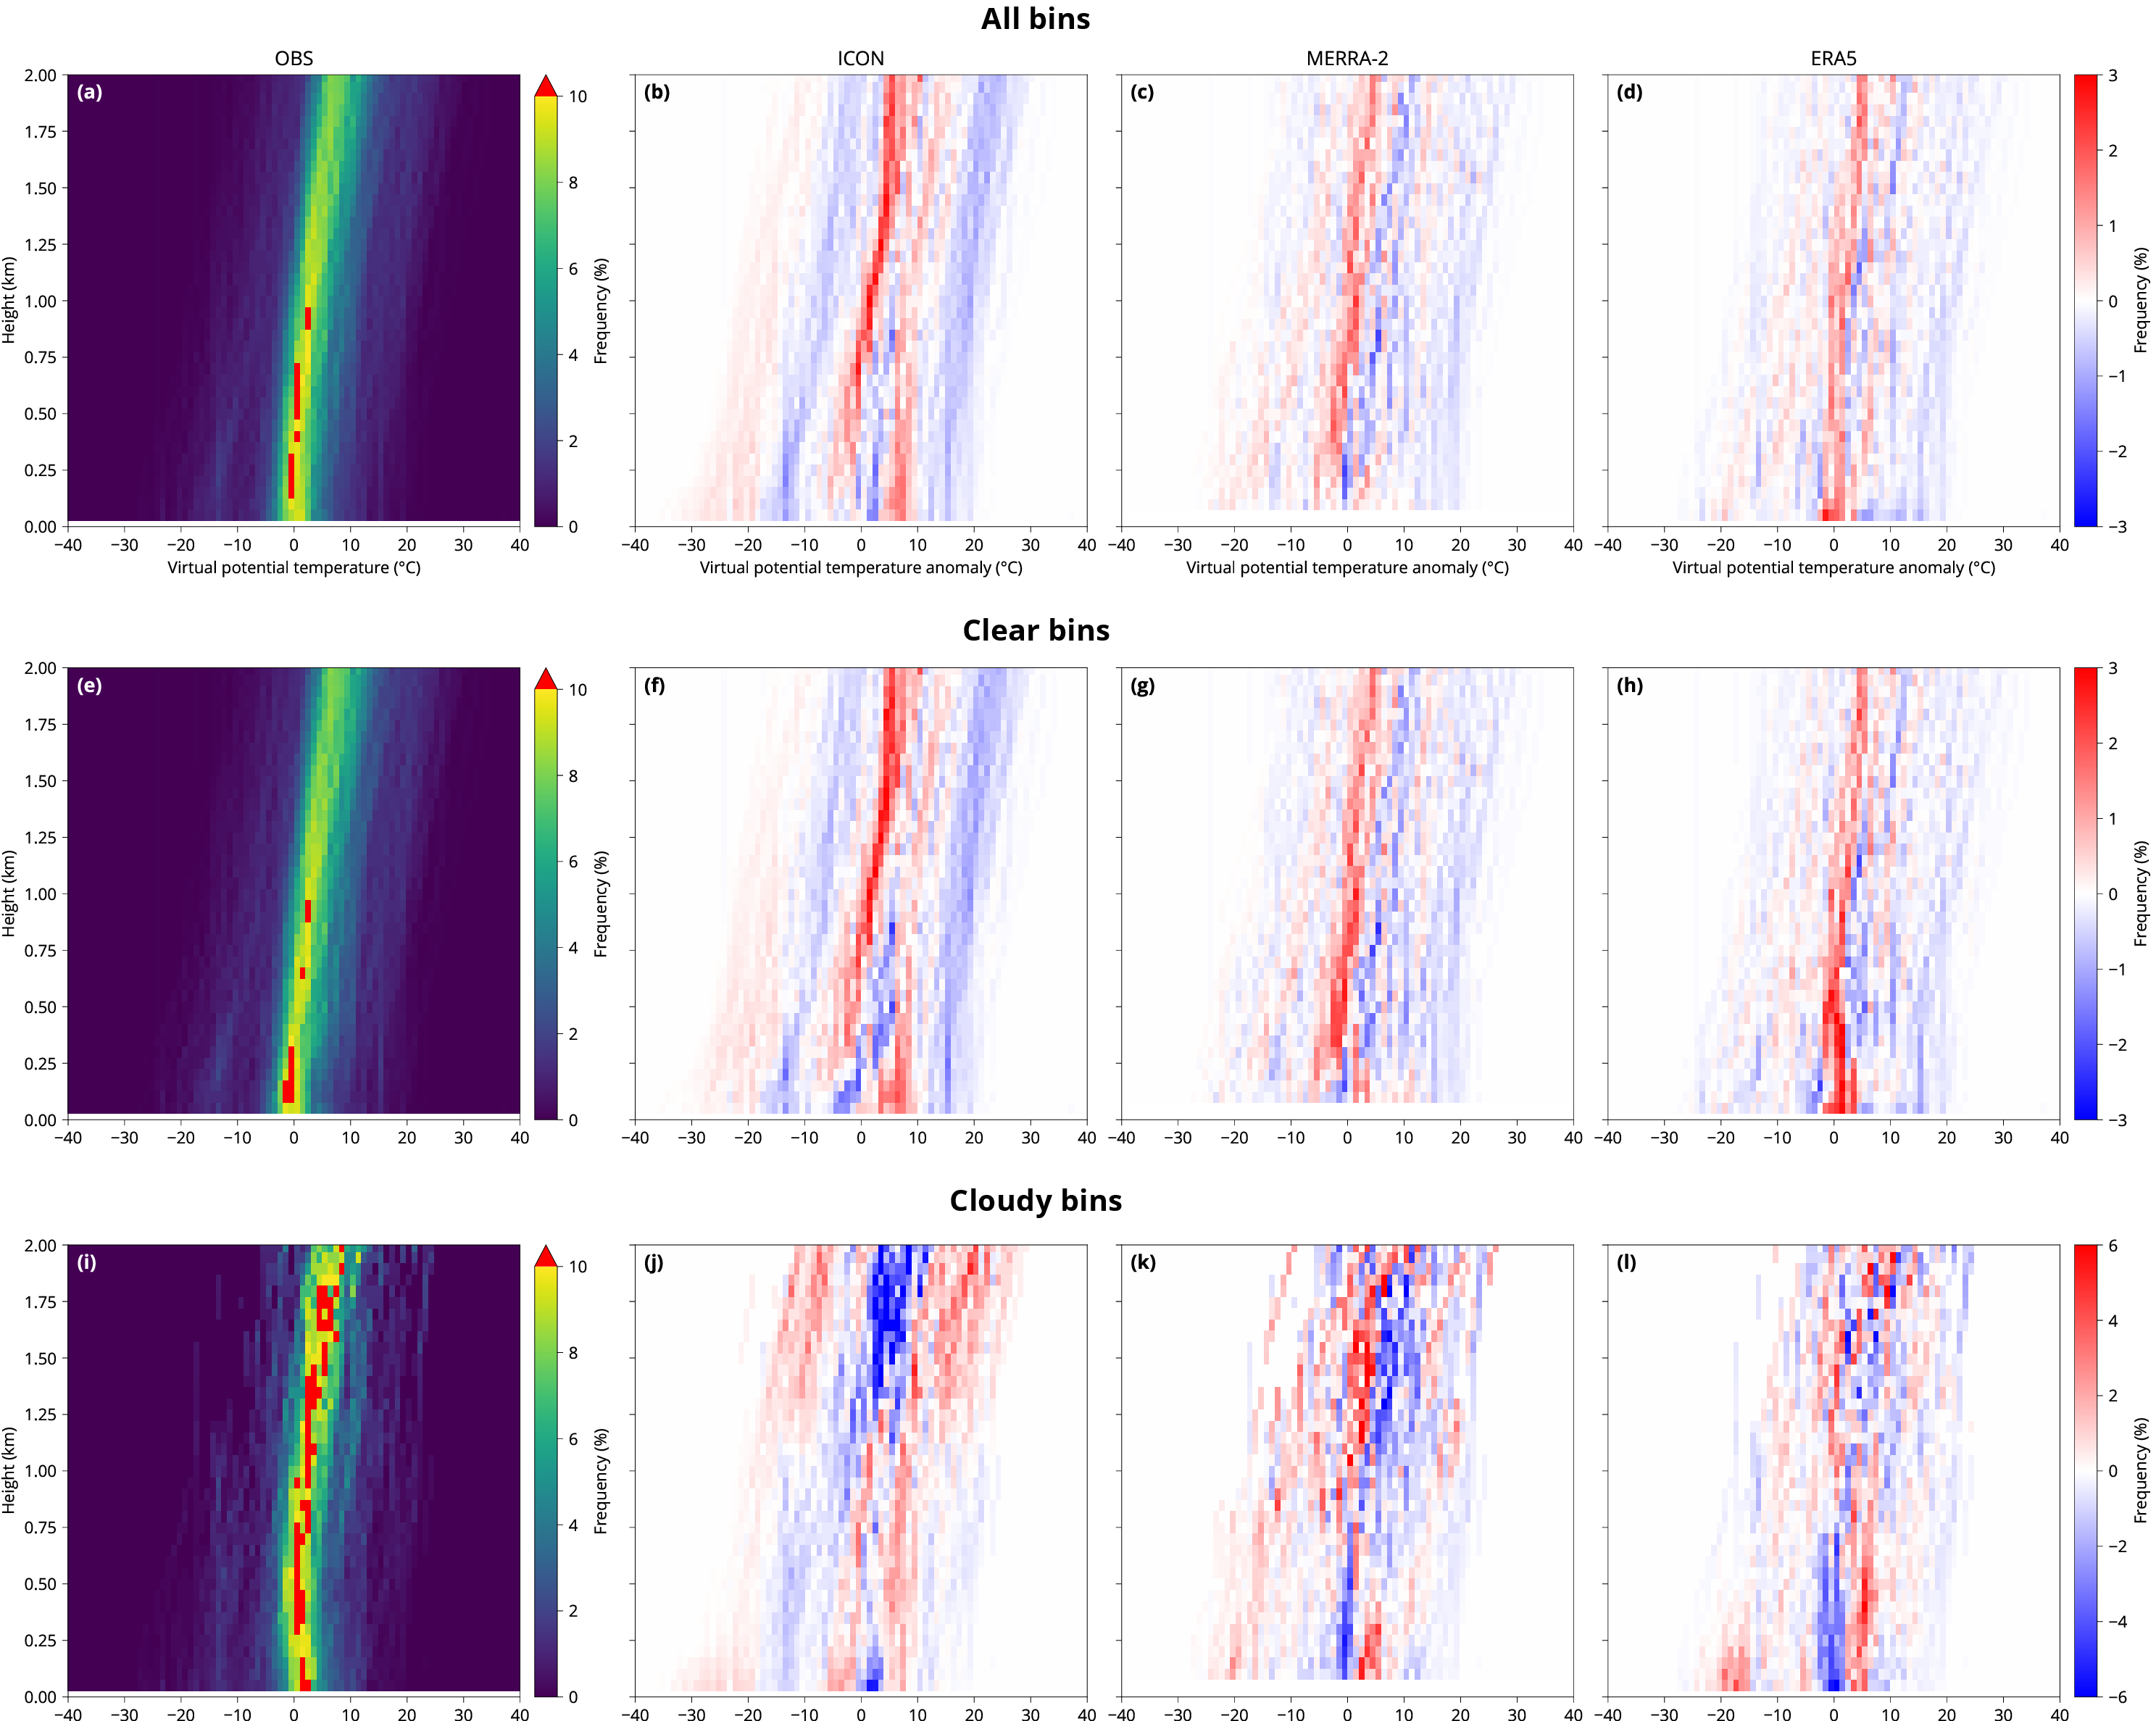
\includegraphics[width=1.2\textwidth]{img/rs_thetav_hist.png}
}
\caption{
The same as Fig.~\ref{fig:rs-hur-hist}, but for virtual potential temperature.
}
\label{fig:rs-thetav-hist}
\end{figure}

\end{document}
